\documentclass[a4paper,12pt]{article}
\usepackage[utf8]{inputenc} % Required for inserting images
\usepackage[Brazil]{babel}%portugues brasileiro
\usepackage[lmargin=3cm,tmargin=3cm,rmargin=2cm,bmargin=2cm]{geometry}%abnt
\usepackage[t1]{fontenc}%ajusta o texto que vem de outra fonte
\usepackage{amsmath,amsthm,amsfonts,amssymb,dsfont,mathtools,blindtext} %pacotes matemáticos
\usepackage{blindtext}
\usepackage{graphicx}

\begin{document}
\maketitle
\section{tipos de árvores}%titulo
\subsection{tipos de árvores 01}%Sessão 1.1

\begin{flushrileft}%margem a esquerda
Também conhecido como “Coração de Boi”, essa espécie pode ser encontrada na Argentina, Paraguai e Brasil, e pode atingir até 18 metros de altura. Sua madeira é utilizada em construção de forros, e para confecção de caixotes, brinquedos e alguns utensílios domésticos. Seus frutos são agradáveis ao paladar humano, entretanto causam disenteria, assim devem ser ingeridos em pequenas porções.
\end{flushrileft}%fechar

\begin{center}%ao centro
\textit{Essa espécie é nativa do Brasil, estando presente principalmente em serras litorâneas} %italico
e restingas presentes nos estados de São Paulo, Rio de Janeiro e parte do território de Minas Gerais. Possui crescimento rápido, podendo atingir entre 2 e 4 metros de altura; a frutificação ocorre entre outubro e dezembro, e sua polpa é levemente ácida.
\end{center}%fechar

\begin{flushright}%margem a direita
\subsection{outras árvores}
Também conhecido como “Abiu Roxo”, essa espécie é nativa da América Central e Antilhas, incluindo o Haiti e Cuba, pode atingir até 18 metros de altura, e é rica em látex. Sua frutificação ocorre entre julho e dezembro, e é uma espécie bastante utilizada para ornamentação.
\end{flushright}

\begin{figure}[ht]
    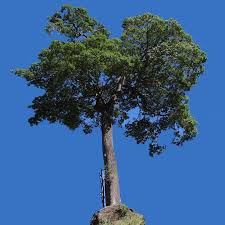
\includegraphics[width=5cm]{arvore.jpeg}
    \caption{Árvore}
    \label{fig0}

lerooolerolerolerolerolero\ref{fig0}
\end{figure}
lero lero lero

\end{document}
